\documentclass[UTF8]{ctexart}
\usepackage{xcolor}
\usepackage{amsmath}
\usepackage{bm}
\usepackage{amssymb}
\usepackage[colorlinks,linkcolor=blue,citecolor=black]{hyperref}
\usepackage{graphicx}
\usepackage{subfigure}
\usepackage{caption}
\usepackage{tocbibind}
\usepackage{geometry}
\usepackage{tikz}
\usetikzlibrary{quotes,angles}

\begin{document}

\section{第一次记录}
\subsection{问题描述}
已知目标和平台在平面 $XOY$ 上运动,$XOY$ 坐标系的刻度单位为千米。

\begin{figure}[h]
    \centering
    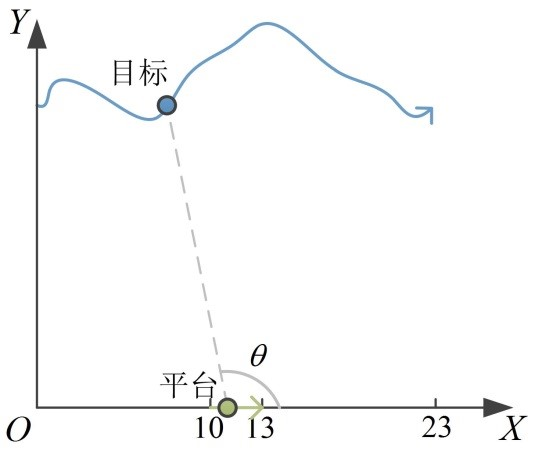
\includegraphics[scale=0.8]{fig1.jpg}
    \caption{目标与平台示意图}
\end{figure}
平台沿 $X$ 轴正向运动,起始位置为 $(10,0)$,终止位置为 $(13,0)$。平台的运动速度为 0.05km/s,因此运动总时间为60s。
目标沿任意曲线运动。平台与目标连线和 $X$ 轴正向的夹角为 $\theta$。

\subsection{建立模型}
假设目标沿 $X$ 轴正向做匀速直线运动,速度 $v=0.38$km/s。则可以看做目标位置不动,平台沿 $X$ 轴负方向以速度 $v=0.33$km/s 做匀速直线运动。则平台相对于静止的目标的位置如下图所示。 \\
\begin{figure}[h]
\centering
\begin{tikzpicture}[scale=0.78]
    \draw[->] (0,0) -- (4.8,0);
    \draw[->] (0,0) -- (0,4.6);
    \draw (0,0) node[below] {$O$};
    \draw (4.8,0) node[below] {$X$};
    \draw (0,4.6) node[left] {$Y$};
    \coordinate (b) at (2,0);
    \coordinate (c) at (2.4,0);
    \coordinate (x) at (0,4);
    \coordinate (d) at (3.2,4);
    \coordinate (e) at (3,0);
    \draw (x) node[left] {$\bm{x}$} -- (b) node[below] {$\bm{b_0}$} -- (c) node[below] {$\bm{b_i}$ } 
    pic [draw, ->, "$\theta_0$", angle radius=1.5mm, angle eccentricity=2.5] {angle = c--b--x};
    \draw (e) -- (c) -- (d) node[right] {$\bm{x_i}$}
    pic [draw,->,"$\theta_i$", angle radius=1.5mm, angle eccentricity=2.5 ] {angle = e--c--d};
    \draw (x)--(d);
    
    \draw[->] (5,2.3) -- (8,2.3);
    \draw (6.5,2.5) node {将目标看做静止};
    
    \draw[->] (8,0) -- (14,0) node[below] {$X$};
    \draw[->] (11,0) -- (11,4.6) node[left] {$Y$};
    \draw (11,0) node[below] {$O$};
    \coordinate (f) at (13,0);
    \coordinate (g) at (10.2,0);
    \coordinate (h) at (11,4);
    \coordinate (j) at (13.5 ,0);
    \draw (j) -- (f) node[below] {$\bm{b_0}$} -- (h) node[left] {$\bm{x}(\bm{x_i})$}
    pic [draw, ->, "$\theta_0$", angle radius=1.5mm, angle eccentricity=2.5] {angle = j--f--h};
    \draw (f) -- (g) node[below] {$\bm{b'_i}$} -- (h)
    pic [draw, ->, "$\theta_i$", angle radius=1.5mm, angle eccentricity=2.5] {angle = f--g--h}; 
\end{tikzpicture}
\caption{平台相对于静止的目标的位置变换}
\end{figure}

如图,假设目标的初始位置坐标为 $\bm{x}=(x_T,y_T)$,每0.1s平台对应的位置分别为 $\bm{b_i}=(b_{ix},b_{iy}), i \in \lbrace 0,1,\cdots,600 \rbrace$,
其中 $\bm{b_0} = (10,0)$。每0.1s平台所测得目标与平台连线和 $X$ 轴正向的夹角为 $\theta_i,i \in \lbrace 0,1,2,\cdots,600 \rbrace$,$\theta_i$ 可测量。将 $\bm{x_i}$ 向 $X$ 轴负方向移动,使之与 $\bm{x}$ 重合。同时将 $\bm{b_i}$
保持对 $\bm{x_i}$ 位置不变进行相对移动,记移动后的点为 $\bm{b'_i}$。根据几何关系可得到
\begin{equation}
    \theta_i = \arctan \frac{y_T-b'_{iy}}{x_T-b'_{ix}}
\end{equation}
由于测量的角度存在噪声,假设每次测量的噪声变量互相独立,且满足高斯分布,即噪声变量 $\eta_i \sim N(0,\sigma^2)$,则测量值 $\tilde{\theta_i}$ 满足
\begin{equation}
    \tilde{\theta_i} = \arctan \frac{y_T-b'_{iy}}{x_T-b'_{ix}} + \eta_i, \quad i \in \lbrace 0,1,\cdots,600 \rbrace
\end{equation}
记 $\bm{\theta} = [\theta_0, \theta_1, \cdots, \theta_{600}]$。然后得到
\begin{equation}
    P(\bm{\theta} | \bm{x}) = \prod\limits_{i = 0}^{600} {\frac{1}{{\sqrt {2\pi } \sigma }}\exp \{  - \frac{{\eta _i^2}}{{2{\sigma ^2}}}\} } 
\end{equation}
求解目标的坐标应得
\begin{equation}
    \begin{split}
        \hat{\bm{x}} =& \mathop {\arg \min }\limits_{({x_T},{y_T})} \frac{\sum\limits_{i=0}^{600} \eta_i^2}{2 \sigma^2} \\
                    =& \mathop {\arg \min}\limits_{(x_T,y_T)} \frac{\sum\limits_{i=0}^{600} (\hat{\theta_i}-\arctan\frac{y_T-b'_{iy}}{x_T-b'_{ix}})^2}{2\sigma^2}
    \end{split}
\end{equation}
当噪声变量足够小时,即 $\eta_i \approx 0$,得到
\begin{equation}
    \begin{split}
    (y_T-b'_{iy})\cos \theta_i - (x_T-b'_{ix})\sin \theta_i \approx 0  \qquad i \in \lbrace 0,1,2,\cdots, 600 \rbrace\\
    \frac{\| \bm{x}-\bm{b'_i}\|}{\sin\theta_i} \approx \frac{\| \bm{x}-\bm{b_0}\|}{\sin\theta_0} \qquad i \in \lbrace 1,2,\cdots,600 \rbrace
    \end{split}
\end{equation}
利用最小二乘法(LS)
\begin{equation}
    \hat{\bm{x}} = \mathop {\arg \min}\limits_{(x_T,y_T)} \sum\limits_{i=0}^{600} [((y_T-b'_{iy})\cos \theta_i - (x_T-b'_{ix})\sin \theta_i)^2 + 
    (\|\bm{x}-\bm{b'_i}\|\sin\theta_i-\|\bm{x}-\bm{b_0}\|\sin\theta_0)^2]
\end{equation}

若已知目标运动速度及运动规律,只需判断目标的初始位置即可确定目标运动的轨迹。


\begin{figure}
    \centering
    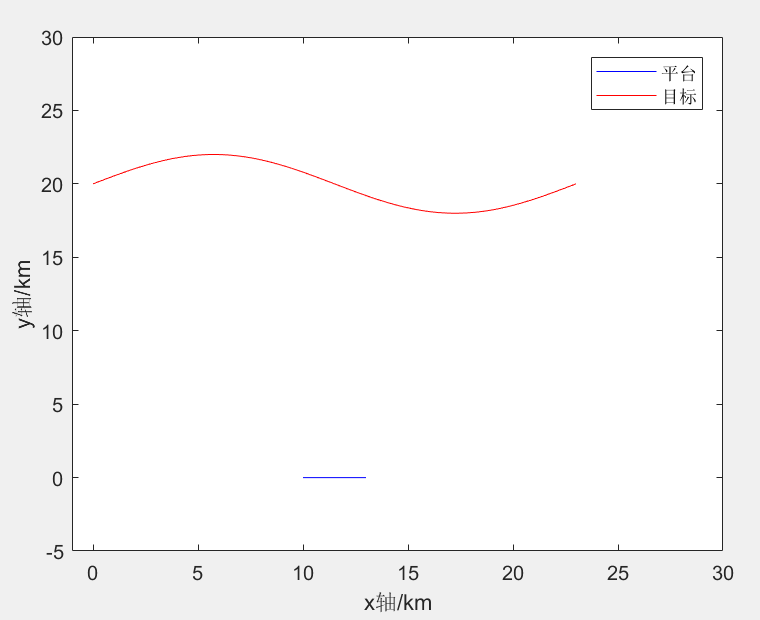
\includegraphics[scale=0.5]{fig2.png}
    \caption{轨迹2运动图像}
\end{figure}
\end{document}